\section{\texorpdfstring{\Gls{spade}}{SPADe} adaptation for an industrial platform}
\label{sec:ch7_SPADeIndustrial}
We have explained the \gls{spade} flow until now assuming that the timing of the implementation is predictable.
However, for an industrial platform, it is difficult to predict the timing analytically (as users have restricted freedom in scheduling due to caching, resource sharing, etc.), and any computed timing is pessimistic.
This section shows how we can apply the \gls{spade} flow even when it is difficult to give tight predictable timing guarantees.
As in Chapter \ref{chap:parallelisation}, the idea is that we use the frequently occurring task execution times instead of the pessimistic \gls{wcet} estimates to obtain temporal bounds. 

Chapter~\ref{chap:parallelisation} explored this idea for a non-pipelined parallelisable implementation. In this chapter, we show that the \gls{spade} adaptation for an industrial platform is relevant for pipelined parallelism as well.
The assumption for implementation is that it is possible to time-trigger tasks either through polling or through interrupt timers in the industrial platform.
We provide validation through a \gls{hil} simulation, showing that we can guarantee control stability for the \gls{spade} design outcomes, despite the fact that the execution-time estimates for tasks used in the \gls{spade} flow are not conservative.

\subsection{\texorpdfstring{\Gls{hil}}{HiL} setting for our case study}
\label{sec:ch7_HiLSetting}
Fig. \ref{fig:ch7_hil} illustrates our \gls{hil} validation setup for \gls{lkas} adapted from \cite{mohamed2019imacs}. It simulates a vehicle with a top look-ahead camera using the Webots \cite{michel2004cyberbotics} physics simulator engine and interacts with an NVIDIA AGX Xavier platform using the \gls{tcpip} protocol. The simulator works in a server-client configuration. Webots acts as the server while the NVIDIA platform acts as the client. The server (Webots) progresses simulation in full synchronisation with the client (NVIDIA AGX Xavier) \cite{nvidiaAGX}. At each simulation step, the camera sensor simulated in Webots generates a raw image containing state information $x[k]$, that is fed to the NVIDIA platform. It executes the sensing ($\taskS$) and control ($\taskC$) tasks to generate control input $u[k]$, which is communicated back to Webots for actuation. After actuation, the simulation progresses to the next step. 

For our evaluation, the camera sensor in Webots is modelled based on the AR1335 \gls{cmos} digital image sensor \cite{camsensor} and is set to a resolution of 720p\footnote{State-of-the-art lane detection algorithms \cite{NvidiaLanenet} operate on low-resolution images. So, we perform our evaluation using downscaled (512$\times$256) sensor images. Our approach is also effective for high-res images.}. The camera frame rate is varied between 30~fps, 60~fps, and 120~fps, depending on the sampling period of the controller. The actuation dynamics are modelled based on \cite{RandyFrank2016}. A lane width of 3.25 m is considered, as per standard road-safety guidelines.
The vehicle is initially positioned with a fixed bias of 15~cm from the lane centre to test the control performance.
The Webots simulation step is set to 1~ms, while the vehicle speed is set to 50~km/hr.
\begin{figure}[t]
\centerline{
    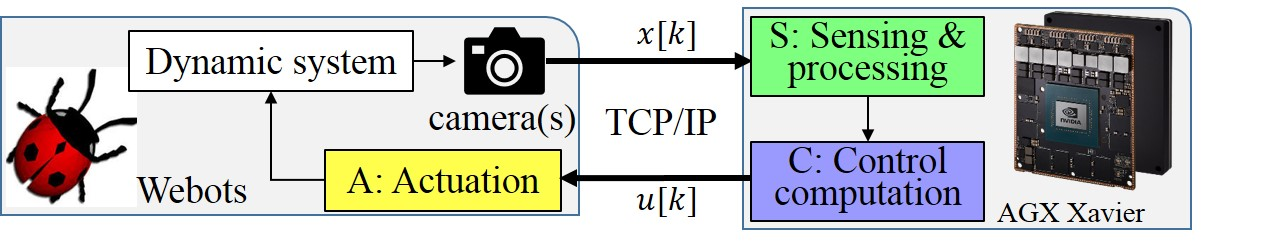
\includegraphics[width=0.8\textwidth]{images/hil.jpg}
    }
    \caption{HiL setting overview with NVIDIA AGX Xavier.}
    \label{fig:ch7_hil}
    %\vspace{-1em}
\end{figure}

\subsection{Platform graph}
We proceed to explain the abstraction we make for the platform graph in Fig.~\ref{fig:ch7_ibc_overview}.
The NVIDIA AGX Xavier platform has a Carmel \gls{cpu} complex with eight cores and a Volta \gls{gpu} with 512 CUDA cores and 64 Tensor cores, as shown in Fig.~\ref{fig:nvidia_platform}.
 Modelling all the \gls{gpu} cores separately may lead to state-space explosion and is inefficient for the dataflow timing and mapping analysis.
Also, the proprietary \gls{gpu} scheduler is closed-source and needs to be accessed through the \gls{cpu}.
The execution times are difficult to predict for the tasks mapped to the \gls{gpu} when there are other shared tasks on the \gls{gpu}.
 Therefore, we abstract and combine the execution times of the tasks mapped to the \gls{gpu} along with the execution time of the \gls{cpu} task that accesses it.
  Thus, the platform allocation is defined based on the total number of \gls{cpu} cores available $\numCoresAvailable$. For the NVIDIA AGX Xavier platform, we have a maximum of eight \gls{cpu} cores, i.e., $\numCoresAvailable=8$.
 
\subsection{\texorpdfstring{\Gls{ibc}}{IBC} graph}
Next, we explain the \gls{ibc} graph of Fig.~\ref{fig:ch7_ibc_overview} used in this experiment and how we populate it with the profiling information. 
We model the \gls{ibc} sensing algorithm using the \gls{ibc} graph illustrated in Fig.~\ref{fig:ch7_hilSADF}. 
 This graph structure is for the approximate setting `S3' of the \gls{ibc} system presented later in Chapter \ref{chap:approximation}.
 The execution time numbers for the actors in the graph and the rates in the channels are obtained by mapping and profiling the \gls{ibc} application on the NVIDIA AGX Xavier platform.
We perform a model-fitting using the profiled timing information to update the execution time of the actors for each workload scenario. 
 The resulting \gls{ibc} \gls{sadf} model is then one of the inputs to the \gls{spade} flow explained in Algorithm~\ref{algo:SPADeFlow}.
 
 For profiling, around 100 images are identified with varying image workloads. We execute each stage in the \gls{lkas} 100 times for every image in the dataset to reduce sensitivity to access locality.
 This helps to characterise the profiling information as a PERT distribution~\cite{adyanthaya2014robustness} for the latency of an iteration of the graph.
 Workload scenarios are classified based on the resulting PERT distribution by identifying regions in the distribution based on occurrence frequency.
 This results in scenario graphs with the same graph structure and channel rates, but  different actor execution times.
 The workload scenarios for this setup are not based on \gls{roi}, as in our running example.
 For the worst-case scenario, we use the worst-case profiling numbers for the execution times of the actors. 
 Other workload scenarios use the best-case, first quartile, median and third quartile profiling data.
 As an example, the model parameters for the workload scenario using third quartile profiling data are $\actorET_{dm}=10.3$~ms,  $\actorET_{dn}=4$~ms, $\actorET_{1}=0.3$~ms, $\actorET_{2}=4.65$~ms, $\actorET_{d}=5$~ms, $\actorET_{p}=1.4$~ms, $\actorET_{m}=0.16$~ms (see Fig.~\ref{fig:ch7_hilSADF}), $\actorET_{\taskC}=0.016$~ms, and $\actorET_{\taskA}=0.5$~ms (assuming single actors \taskC and \taskA for the control compute and actuation tasks).
Workload scenarios may also be classified based on other parameters, like \gls{roi} in the running example.
Our previous work~\cite{mohamed2020scenario} details the case where the workload scenarios are classified based on different operating modes of an application due to environmental conditions. Here, we use the observed overall latency of the sensing, because it is difficult to predict execution times on the considered platform based on other parameters. 

\subsection{\texorpdfstring{\Gls{spade}}{SPADe} flow, \texorpdfstring{\gls{dse}}{DSE} and \texorpdfstring{\gls{hil}}{HiL} validation}
Once we have the \gls{ibc} \gls{sadf} model with the profiling information for every workload scenario, the rest of the steps in the \gls{spade} flow follows Algorithm~\ref{algo:SPADeFlow}.
A \gls{dse} is performed for different implementation choices  $\numCoresParallel$ and $\numPipes$ (as explained in Section~\ref{sec:ch7_DSE}).
A \gls{dse} involves analytical computation of \gls{gm} and \gls{pm} (in Matlab) for the different implementation choices (results are shown in Fig.~\ref{fig:ch7_Pareto_HiL}). 
We consider three given platform allocations - single-core, four cores and eight cores, i.e., $\numCoresAvailable=1,4,8$. The implementation choices with the highest \gls{gm} and \gls{pm} are Pareto-optimal.

\begin{figure}[t]
\centerline{
    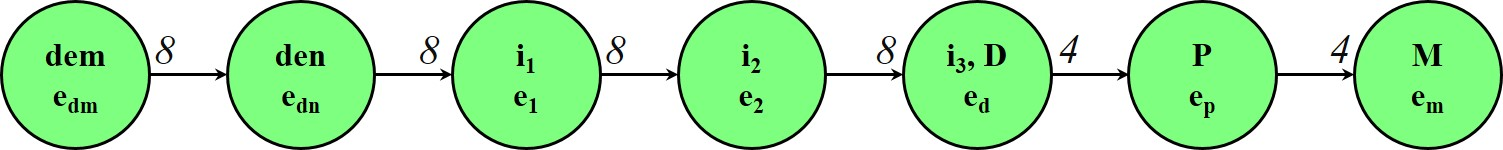
\includegraphics[width=\textwidth]{images/HiL_GS.jpg}
    }
    \caption{\Gls{lkas} \gls{ibc} graph of the sensing algorithm implementation derived from~\cite{de2020approximation}. The actors are: dem - demosaicing; den - denoising; i$_{1,2,3}$ - abstract colour mapping and white balancing, tone mapping, and compression; and D-P-M model the lane detection, processing and merging tasks. The output is the lateral deviation $\yL$.}
    \label{fig:ch7_hilSADF}
    %\vspace{-1em}
\end{figure}

The results in Fig.~\ref{fig:ch7_Pareto_HiL} show that parallelising as much as possible gives the best result, i.e. the configurations $<4,4,1>$ and $<8,8,1>$ have the best \gls{gm} and \gls{pm}. The configurations $<4,4,2>$ and $<8,4,2>$ have similar \gls{gm} and \gls{pm} and can be considered for further analysis. 
The results confirm the earlier conclusion of Section \ref{sec:ch7_DSE} that parallelisation should be prioritised over pipelining. In this case, pipelining does not have any added value ($\numPipes=1$ in both Pareto-optimal configurations), because the \gls{lkas} implementation is highly parallelisable.
For applications with a lower degree of parallelism, e.g., when maximum parallelism is achieved with 4 cores and $\numCoresAvailable=8$, this would likely not be the case. In such a case, we can use the additional four cores for an additional pipe, implying that configuration $<8,4,2>$ would have been ideal.

Next, we validate the Pareto-optimal implementation choices in the \gls{hil} setting of Section~\ref{sec:ch7_HiLSetting} for control stability, considering both parallelism and pipelining together. 
Recall that the \gls{spade} flow has a built-in stability check for the system configurations considering the initial system model.
However, the actual \gls{lkas} implementation has to cater to different environment conditions, noise levels, and model uncertainties.
\Gls{hil} validation is often used to simulate the designed system configurations under real-life environment conditions. Therefore, we also perform a \gls{hil} validation experiment.
From the experiment, we observe that stability of the implementation choices of the closed-loop system is confirmed.
We can moreover verify that the order of the control system performance obtained in \gls{hil} conforms to the \gls{gm} and \gls{pm} predictions. 
As explained, we rely on analytical metrics \gls{gm} and \gls{pm} to select our design points.
The \gls{mse} and \gls{st} comparisons are omitted as performing an exhaustive, fair simulation for even a single design point is too compute intensive. But the \gls{dse} performed with the \gls{spade} flow and the \gls{hil} validation of the results show that \gls{spade} can be adopted for industrial platforms.

\begin{figure}[ht]
\centerline{
    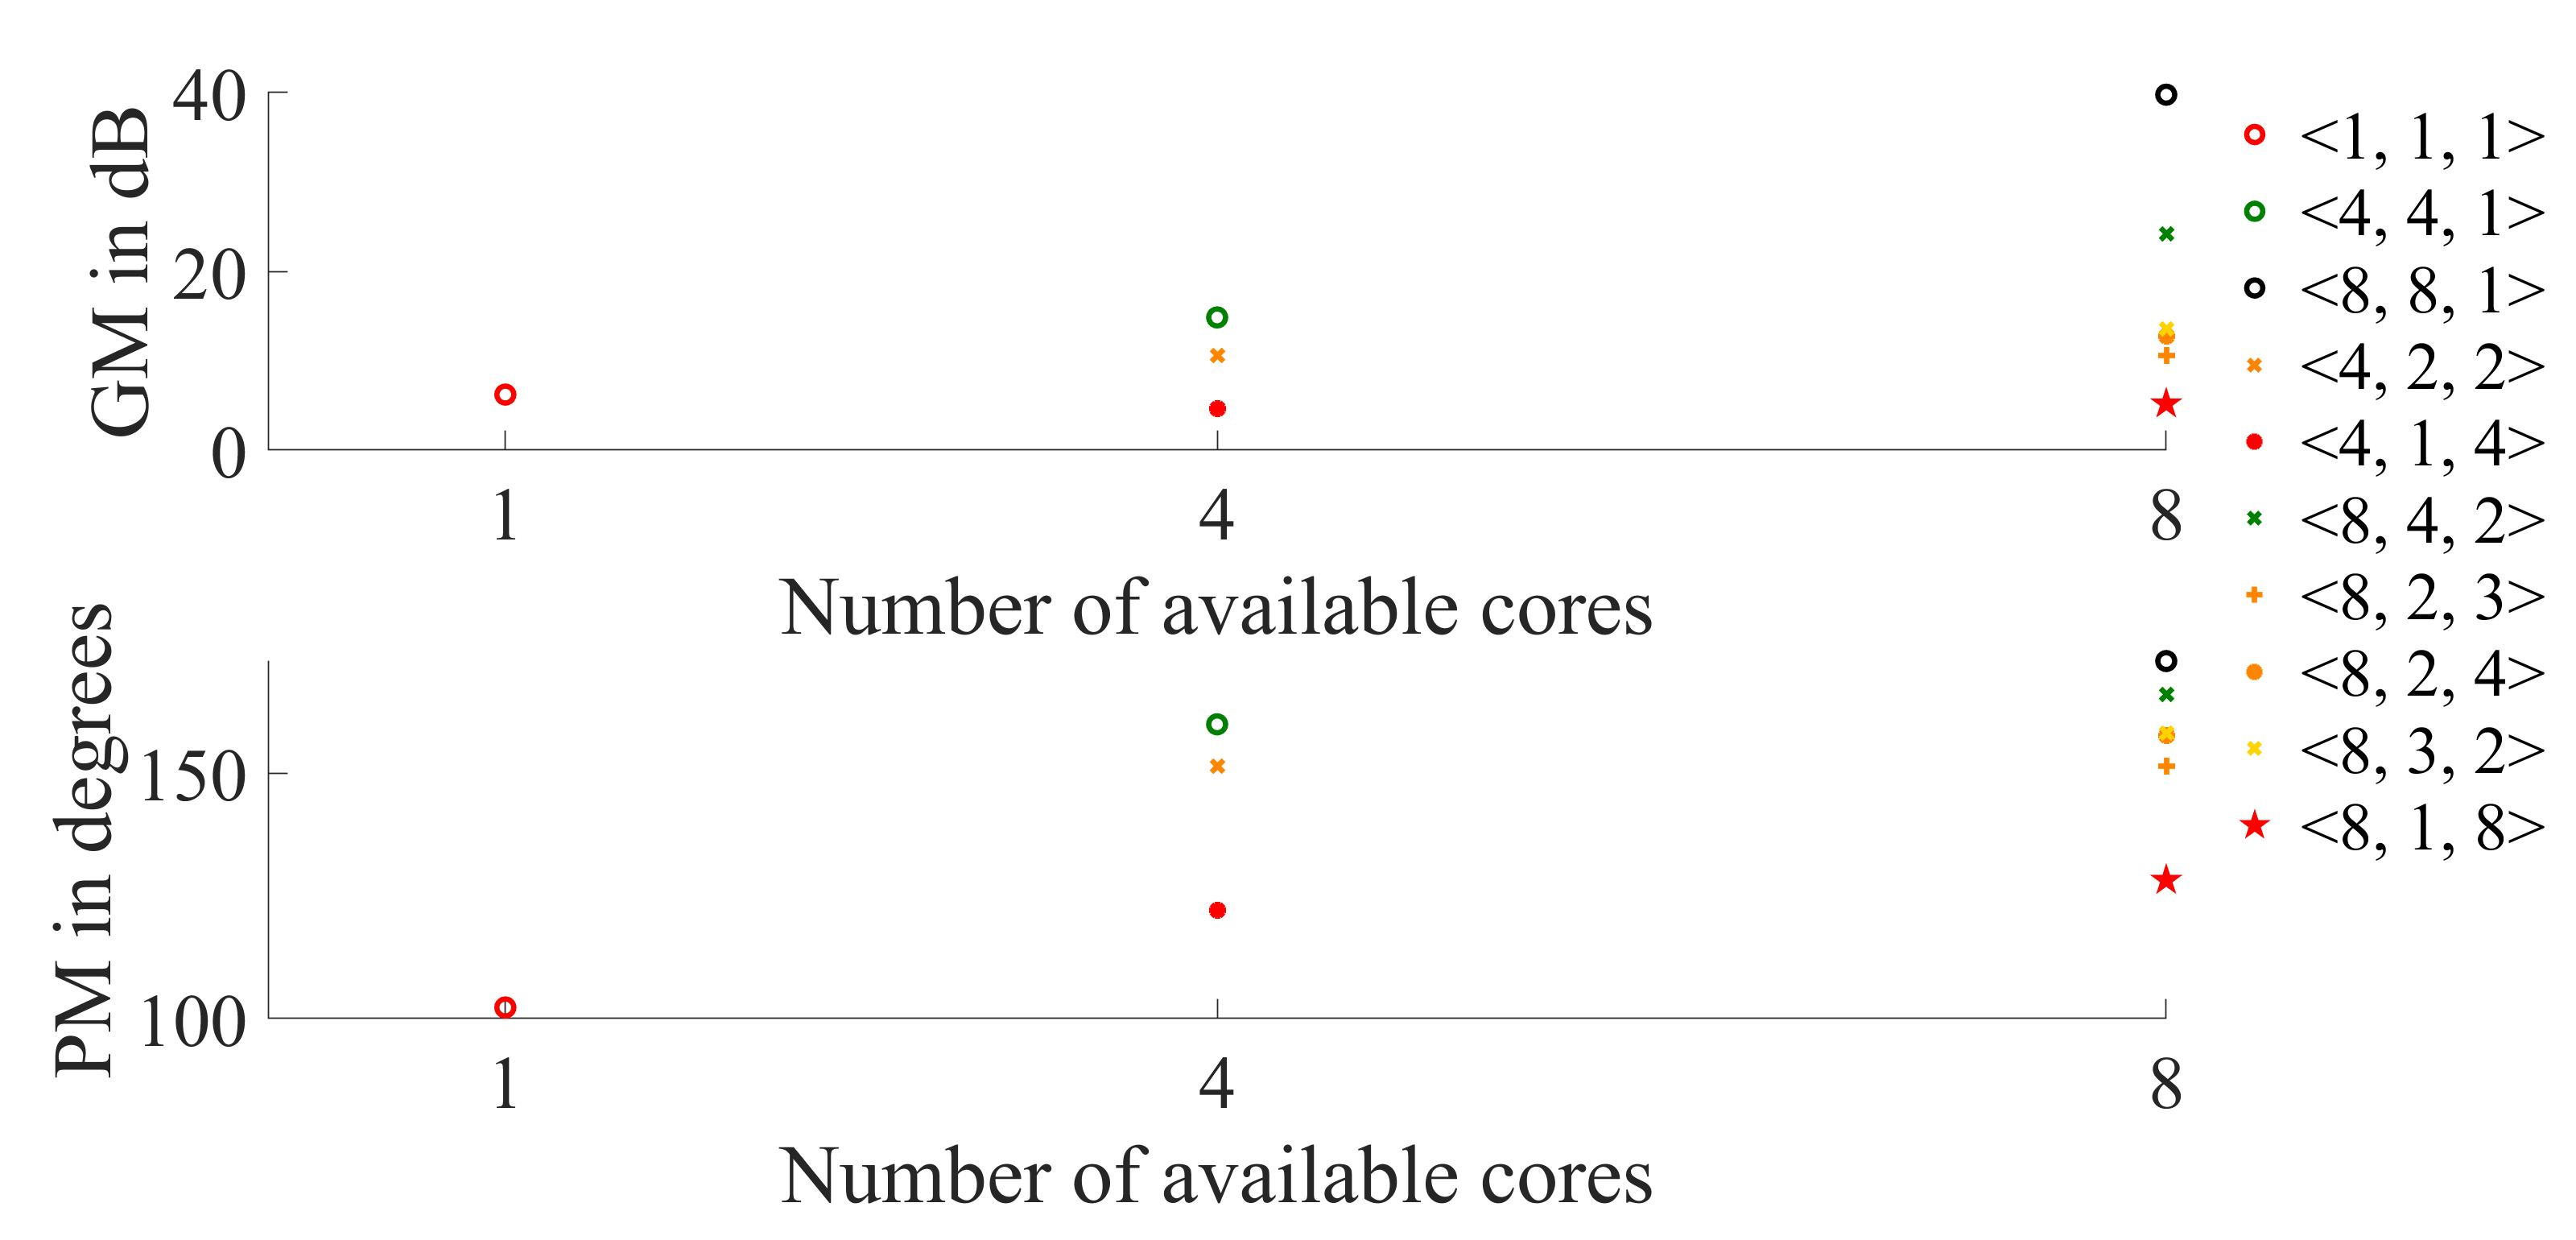
\includegraphics[width=0.8\textwidth]{images/ParetoHiL.jpg}
    }
    \caption{Pareto-plot for \gls{gm} and \gls{pm} vs $\numCoresAvailable$. The legend denotes \mbox{$<\numCoresAvailable,\ \numCoresParallel, \numPipes>$}.}
    \label{fig:ch7_Pareto_HiL}
    %\vspace{-1em}
\end{figure}